% Asset ID: FAS2RecurrenceRelationshipsTikZ-002
% Source: Uploaded recurrence relations transcript, zombie and bacteria recurrence examples.
% Related lesson section: # 9. Visual Asset Integration and # 11. Worked Examples
% Used placeholder:
% [VISUAL PLACEHOLDER: FAS2RecurrenceRelationshipsTikZ-002 | Source: Uploaded transcript zombie and bacteria examples | Insert from tikz/FAS2RecurrenceRelationshipsTikZ-002.tex | Purpose: Show discrete-time dependency in population recurrence models.]
% Purpose: Show discrete-time dependency in population recurrence models, including bacteria growth differences and zombie population dependence.
% Creation notes:
% Panel A preserves the bacteria reasoning:
% current increase = 2(previous increase), so b_n - b_{n-1} = 2(b_{n-1} - b_{n-2}), hence b_n = 3b_{n-1} - 2b_{n-2}.
% Panel B preserves the zombie reasoning:
% previous population remains, each zombie bites one human, and zombies more than one day old bite an additional three humans.
% Thus P_n = P_{n-1} + P_{n-1} + 3P_{n-2} = 2P_{n-1} + 3P_{n-2}.

\documentclass[tikz,border=8pt]{standalone}

\usepackage{amsmath}
\usepackage{xcolor}
\usetikzlibrary{arrows.meta,positioning,calc,decorations.pathreplacing}

\definecolor{Canvas}{HTML}{FAF9F6}
\definecolor{Ivory}{HTML}{FFFFF0}
\definecolor{Line}{HTML}{E5E5EA}
\definecolor{Gold}{HTML}{C5A059}
\definecolor{DeepGold}{HTML}{D4AF37}
\definecolor{SoftPink}{HTML}{FBEFEF}
\definecolor{Text}{HTML}{2C2C2E}

\begin{document}

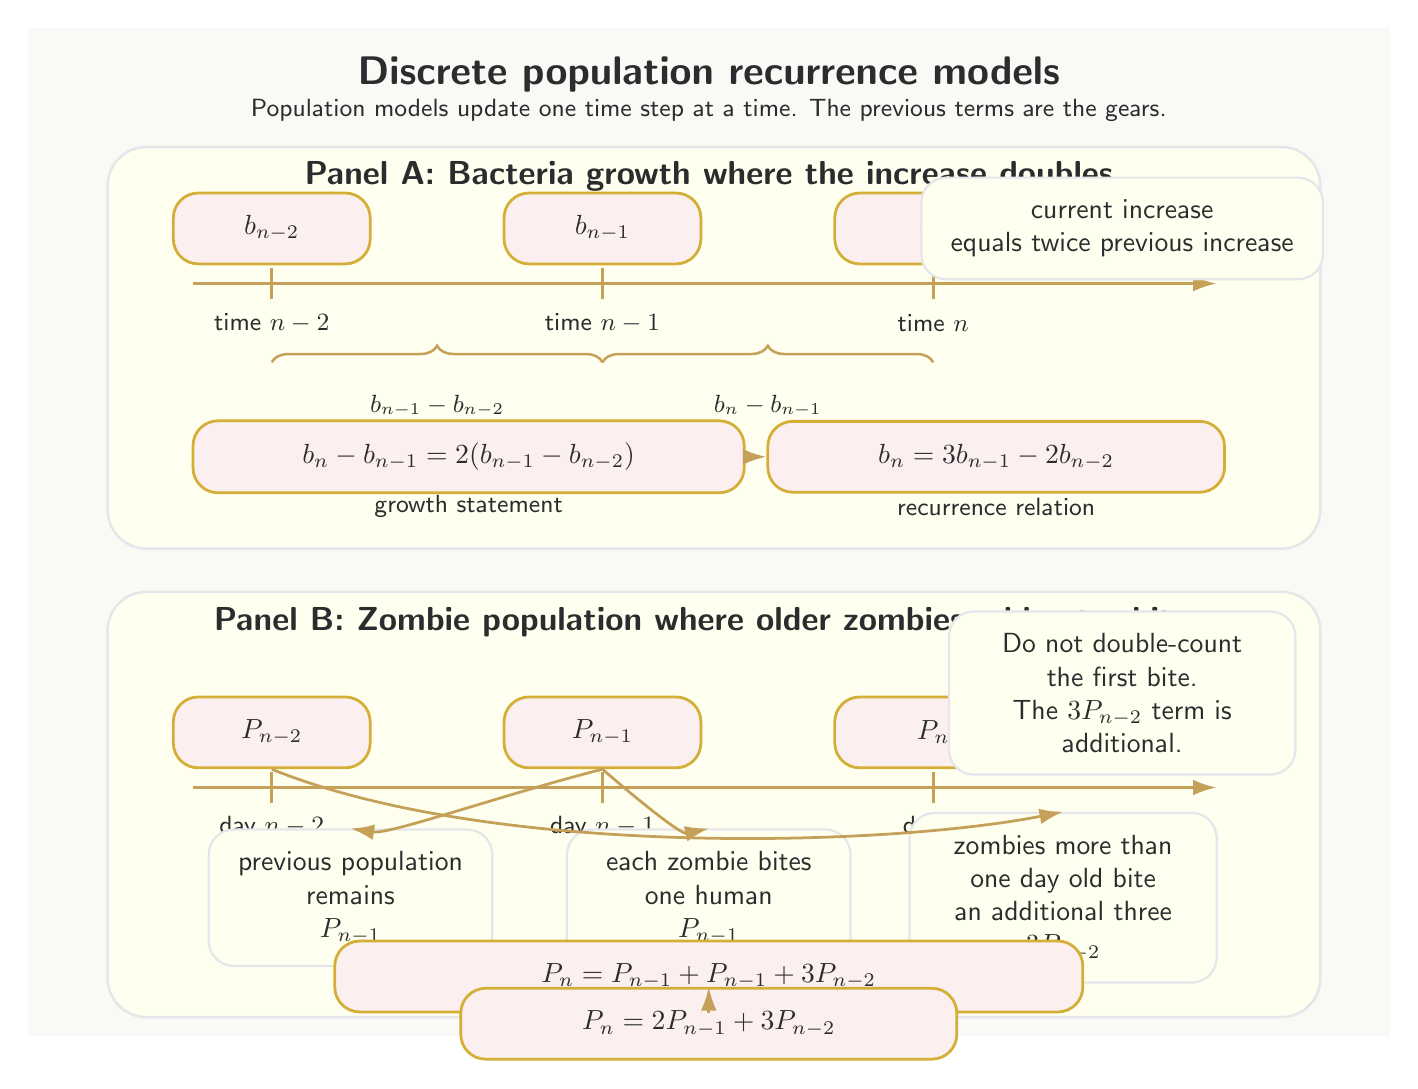
\begin{tikzpicture}[
    font=\sffamily,
    text=Text,
    panel/.style={
        rounded corners=14pt,
        draw=Line,
        line width=0.9pt,
        fill=Ivory,
        inner sep=10pt
    },
    box/.style={
        rounded corners=9pt,
        draw=Line,
        line width=0.8pt,
        fill=Ivory,
        align=center,
        inner sep=8pt,
        minimum height=0.9cm
    },
    highlight/.style={
        rounded corners=9pt,
        draw=DeepGold,
        line width=1pt,
        fill=SoftPink,
        align=center,
        inner sep=8pt,
        minimum height=0.9cm
    },
    arrow/.style={
        -{Latex[length=3mm,width=2mm]},
        line width=1pt,
        draw=Gold
    },
    timearrow/.style={
        -{Latex[length=3mm,width=2mm]},
        line width=1.1pt,
        draw=Gold
    },
    tick/.style={
        draw=Gold,
        line width=1pt
    },
    labeltext/.style={
        font=\sffamily\small,
        text=Text,
        align=center
    },
    mathtext/.style={
        font=\sffamily\large,
        text=Text,
        align=center
    }
]

% Background
\fill[Canvas] (-0.9,-6.3) rectangle (16.4,6.5);

% Title
\node[font=\sffamily\bfseries\Large, text=Text] at (7.75,5.9)
{Discrete population recurrence models};

\node[font=\sffamily\small, text=Text, align=center] at (7.75,5.45)
{Population models update one time step at a time. The previous terms are the gears.};

% Panels
\node[panel, minimum width=15.4cm, minimum height=5.1cm, anchor=north west] at (0.1,5.0) {};
\node[panel, minimum width=15.4cm, minimum height=5.4cm, anchor=north west] at (0.1,-0.65) {};

% Panel headings
\node[font=\sffamily\bfseries\large, text=Text] at (7.75,4.62)
{Panel A: Bacteria growth where the increase doubles};

\node[font=\sffamily\bfseries\large, text=Text] at (7.75,-1.05)
{Panel B: Zombie population where older zombies add extra bites};

% ===========================
% Panel A: bacteria timeline
% ===========================

% Timeline
\draw[timearrow] (1.2,3.25) -- (14.2,3.25);

\foreach \x/\lab in {2.2/{n-2},6.4/{n-1},10.6/{n}} {
    \draw[tick] (\x,3.05) -- (\x,3.45);
    \node[labeltext] at (\x,2.75) {time \(\lab\)};
}

\node[highlight, minimum width=2.5cm] (bn2) at (2.2,3.95) {\(\displaystyle b_{n-2}\)};
\node[highlight, minimum width=2.5cm] (bn1) at (6.4,3.95) {\(\displaystyle b_{n-1}\)};
\node[highlight, minimum width=2.5cm] (bn) at (10.6,3.95) {\(\displaystyle b_n\)};

% Difference braces
\draw[decorate, decoration={brace, amplitude=6pt}, draw=Gold, line width=0.9pt]
(2.2,2.25) -- (6.4,2.25)
node[midway, below=8pt, labeltext] {\(\displaystyle b_{n-1}-b_{n-2}\)};

\draw[decorate, decoration={brace, amplitude=6pt}, draw=Gold, line width=0.9pt]
(6.4,2.25) -- (10.6,2.25)
node[midway, below=8pt, labeltext] {\(\displaystyle b_n-b_{n-1}\)};

\node[box, minimum width=5.1cm] at (13.0,3.95)
{current increase\\equals twice previous increase};

\node[highlight, minimum width=7.0cm] (eqA) at (4.7,1.05)
{\(\displaystyle b_n-b_{n-1}=2(b_{n-1}-b_{n-2})\)};

\node[highlight, minimum width=5.8cm] (eqB) at (11.4,1.05)
{\(\displaystyle b_n=3b_{n-1}-2b_{n-2}\)};

\draw[arrow] (eqA.east) -- (eqB.west);

\node[labeltext] at (4.7,0.42)
{growth statement};

\node[labeltext] at (11.4,0.42)
{recurrence relation};

% ===========================
% Panel B: zombie model
% ===========================

% Zombie time boxes
\node[highlight, minimum width=2.5cm] (pn2) at (2.2,-2.45) {\(\displaystyle P_{n-2}\)};
\node[highlight, minimum width=2.5cm] (pn1) at (6.4,-2.45) {\(\displaystyle P_{n-1}\)};
\node[highlight, minimum width=2.5cm] (pnn) at (10.6,-2.45) {\(\displaystyle P_n\)};

\draw[timearrow] (1.2,-3.15) -- (14.2,-3.15);

\foreach \x/\lab in {2.2/{n-2},6.4/{n-1},10.6/{n}} {
    \draw[tick] (\x,-3.35) -- (\x,-2.95);
    \node[labeltext] at (\x,-3.65) {day \(\lab\)};
}

\node[box, minimum width=3.6cm] (remain) at (3.2,-4.55)
{previous population\\remains\\\(\displaystyle P_{n-1}\)};

\node[box, minimum width=3.6cm] (firstbite) at (7.75,-4.55)
{each zombie bites\\one human\\\(\displaystyle P_{n-1}\)};

\node[box, minimum width=3.9cm] (extra) at (12.25,-4.55)
{zombies more than\\one day old bite\\an additional three\\\(\displaystyle 3P_{n-2}\)};

\draw[arrow] (pn1.south) .. controls (5.1,-3.25) and (3.7,-3.75) .. (remain.north);
\draw[arrow] (pn1.south) .. controls (6.9,-3.35) and (7.4,-3.75) .. (firstbite.north);
\draw[arrow] (pn2.south) .. controls (5.0,-4.05) and (10.0,-3.9) .. (extra.north);

\node[highlight, minimum width=9.5cm] (zomEq1) at (7.75,-5.55)
{\(\displaystyle P_n=P_{n-1}+P_{n-1}+3P_{n-2}\)};

\node[highlight, minimum width=6.3cm] (zomEq2) at (7.75,-6.15)
{\(\displaystyle P_n=2P_{n-1}+3P_{n-2}\)};

\draw[arrow] (zomEq1.south) -- (zomEq2.north);

% Caution note
\node[box, minimum width=4.4cm] at (13.0,-1.95)
{Do not double-count\\the first bite.\\The \(3P_{n-2}\) term is\\additional.};

\end{tikzpicture}

\end{document}
